\chapter{Slučajevi upotrebe aplikacije Interpres}\label{ch:slucajevi_upotrebe}


\renewcommand{\labelenumii}{\arabic{enumi}.\arabic{enumii}}
\renewcommand{\labelenumiii}{\arabic{enumi}.\arabic{enumii}.\arabic{enumiii}}
\renewcommand{\labelenumiv}{\arabic{enumi}.\arabic{enumii}.\arabic{enumiii}.\arabic{enumiv}}

Razvoj softvera iterativnom metodom diktira i uređivanje prevoda za aplikaciju. Na kraju svakog 
ciklusa, programeri obaveste prevodioce da su završili kako bi prevodioci mogli da započnu svoj 
ciklus prevođenja. 

U ovom poglavlju će biti opisani slučajevi upotrebe. Na dijagramu \ref{fig:slucajevi_upotrebe} je 
prikazana šira slika svih slučajeva upotrebe. 

\begin{figure}[H]
    \centering
    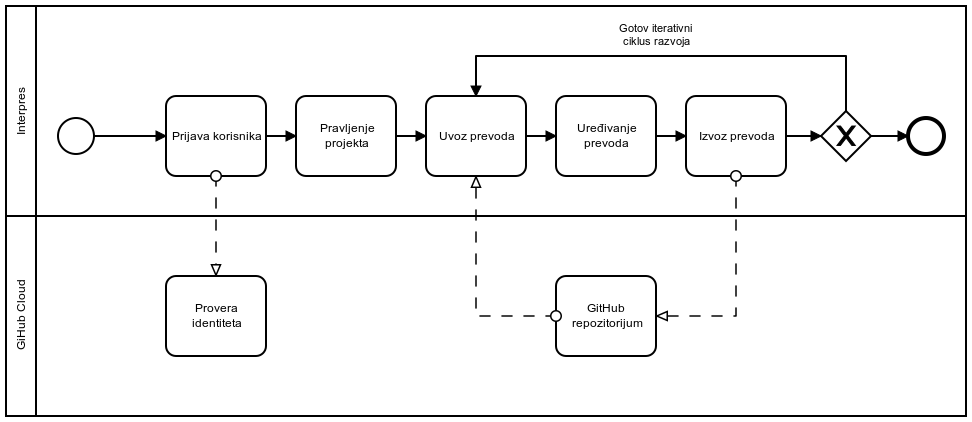
\includegraphics[width=1\textwidth]{slucajevi_upotrebe}
    \caption{BPMN dijagram slučajeva upotrebe}
    \label{fig:slucajevi_upotrebe}
\end{figure}

%%%%%%%%%%%%%%%%%%%%%%
\section{Prijava korisnika uz pomoć GitHub IdP}

\textbf{Kratak opis}: Korisnik se prijavljuje sa sopstvenim kredencijalima

\textbf{Učesnici}: Korisnik

\textbf{Postuslov}: Korisnik je prijavljen

\textbf{Glavni tok}:
\begin{enumerate}
    \item Korisnik klikne na dugme za prijavu
    \item Sistem šalje zahtev prema \textit{Gateway}-u za prijavu
    \item \textit{Gateway} vraća preusmeravanje (302 \textit{Redirect}) na stranicu za prijavu 
    provajdera identiteta (u ovom slučaju \textit{GitHub})
    \item Šalje se zahtev za dobijanje stranice za prijavu provajdera 
    identiteta
    \item \textit{GitHub} šalje stranicu za prijavu korisnika
    \item Korisnik unosi svoje kredencijale
    \item Korisnik šalje zahtev za prijavu klikom na dugme
    \item \textit{GitHub} dobija podatke za prijavu i nakon uspešnog prijavljivanja 
    šalje kod za pristup veb aplikaciji
    \item Veb aplikacija prosleđuje \textit{Gateway}-u kod za pristup
    \item \textit{Gateway}, uz zahtev za dobijanje podataka o korisniku, prosleđuje 
    kod za pristup \textit{GitHub}-u 
    \item \textit{GitHub Gateway}-u vraća podatke o korisniku
    \item Na osnovu dobijenih podataka \textit{Gateway} generiše \textit{JWT} token
    \item \textit{Gateway} šalje \textit{JWT} token veb aplikaciji
    \item Veb aplikacija omogućava prikaz zaštićene stranice korisniku 
    i čuva \textit{JWT} token za buduće komunikacije
\end{enumerate}

\begin{figure}[H]
    \centering
    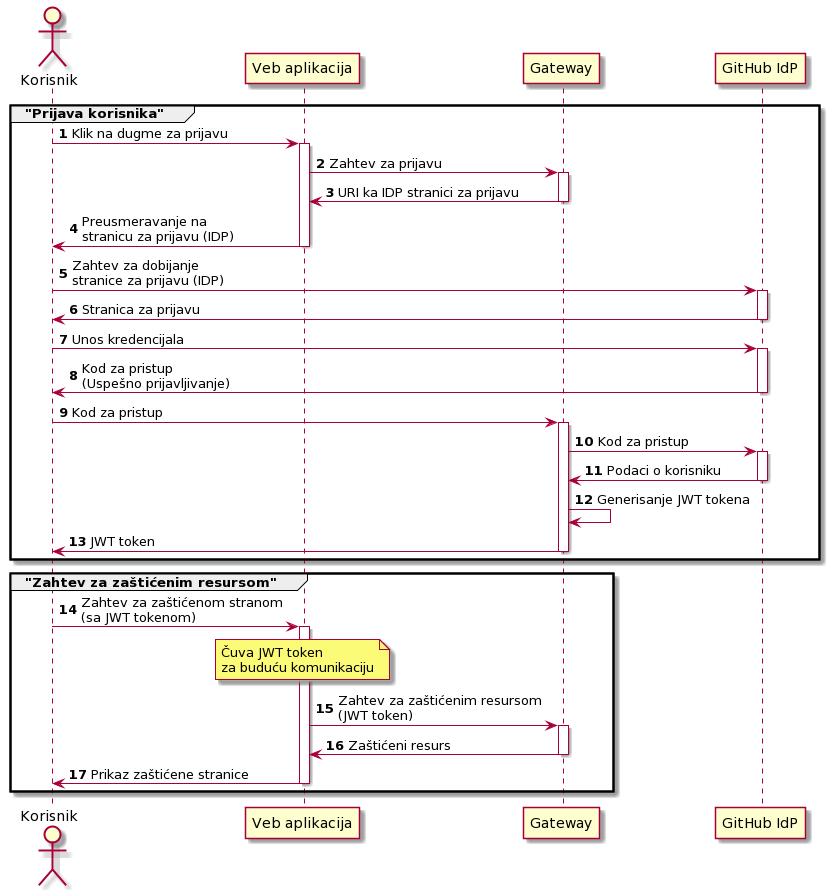
\includegraphics[width=1\textwidth]{prijava_korisnika}
    \caption{Dijagram sekvence -- prijava korisnika}
\end{figure}


%%%%%%%%%%%%%%%%%%%%%%
\section{Pravljenje projekta}

\textbf{Kratak opis}: Prevodilac ima mogućnost da napravi novi projekat

\textbf{Učesnici}: Prevodilac

\textbf{Postuslov}: Projekat je napravljen

\textbf{Glavni tok}:
\begin{enumerate}
    \item Sistem prikazuje opciju za pravljenje novog projekta
    \item Prevodilac bira akciju za pravljenje novog projekta
    \item Sistem prikazuje formu sa tekstualnim poljima za unos podataka o projektu
    \item Prevodilac unosi 
    \begin{itemize}
        \item naziv projekta
        \item vlasnika \textit{GitHub} repozitorijuma
        \item \textit{GitHub} repozitorijum
        \item putanju na kojoj će se čuvati fajlovi sa prevodima i
        \item skup jezika za koje su potrebni prevodi.
    \end{itemize}
    \item Prevodilac klikne na dugme za testiranje konekcije
    \begin{itemize}
        \item Ukoliko su podešavanja pravilno unešena i \textit{GitHub} aplikacija uspešno instalirana u repozitorijum,
        sistem prikazuje uspešnu poruku zajedno sa jezicima koje je pronašao u repozitorijumu
        \item Ukoliko podešavanja nisu pravilno unešena ili \textit{GitHub} aplikacija nije uspešno instalirana u repozitorijum,
        sistem prikazuje poruku sa greškom.
    \end{itemize}
    \item Prevodilac klikne na dugme za pravljenje projekta
    \item Sistem čuva projekat
    \item Sistem prevodiocu vraća stranicu sa podacima o projektu
\end{enumerate}

\begin{figure}[H]
    \centering
    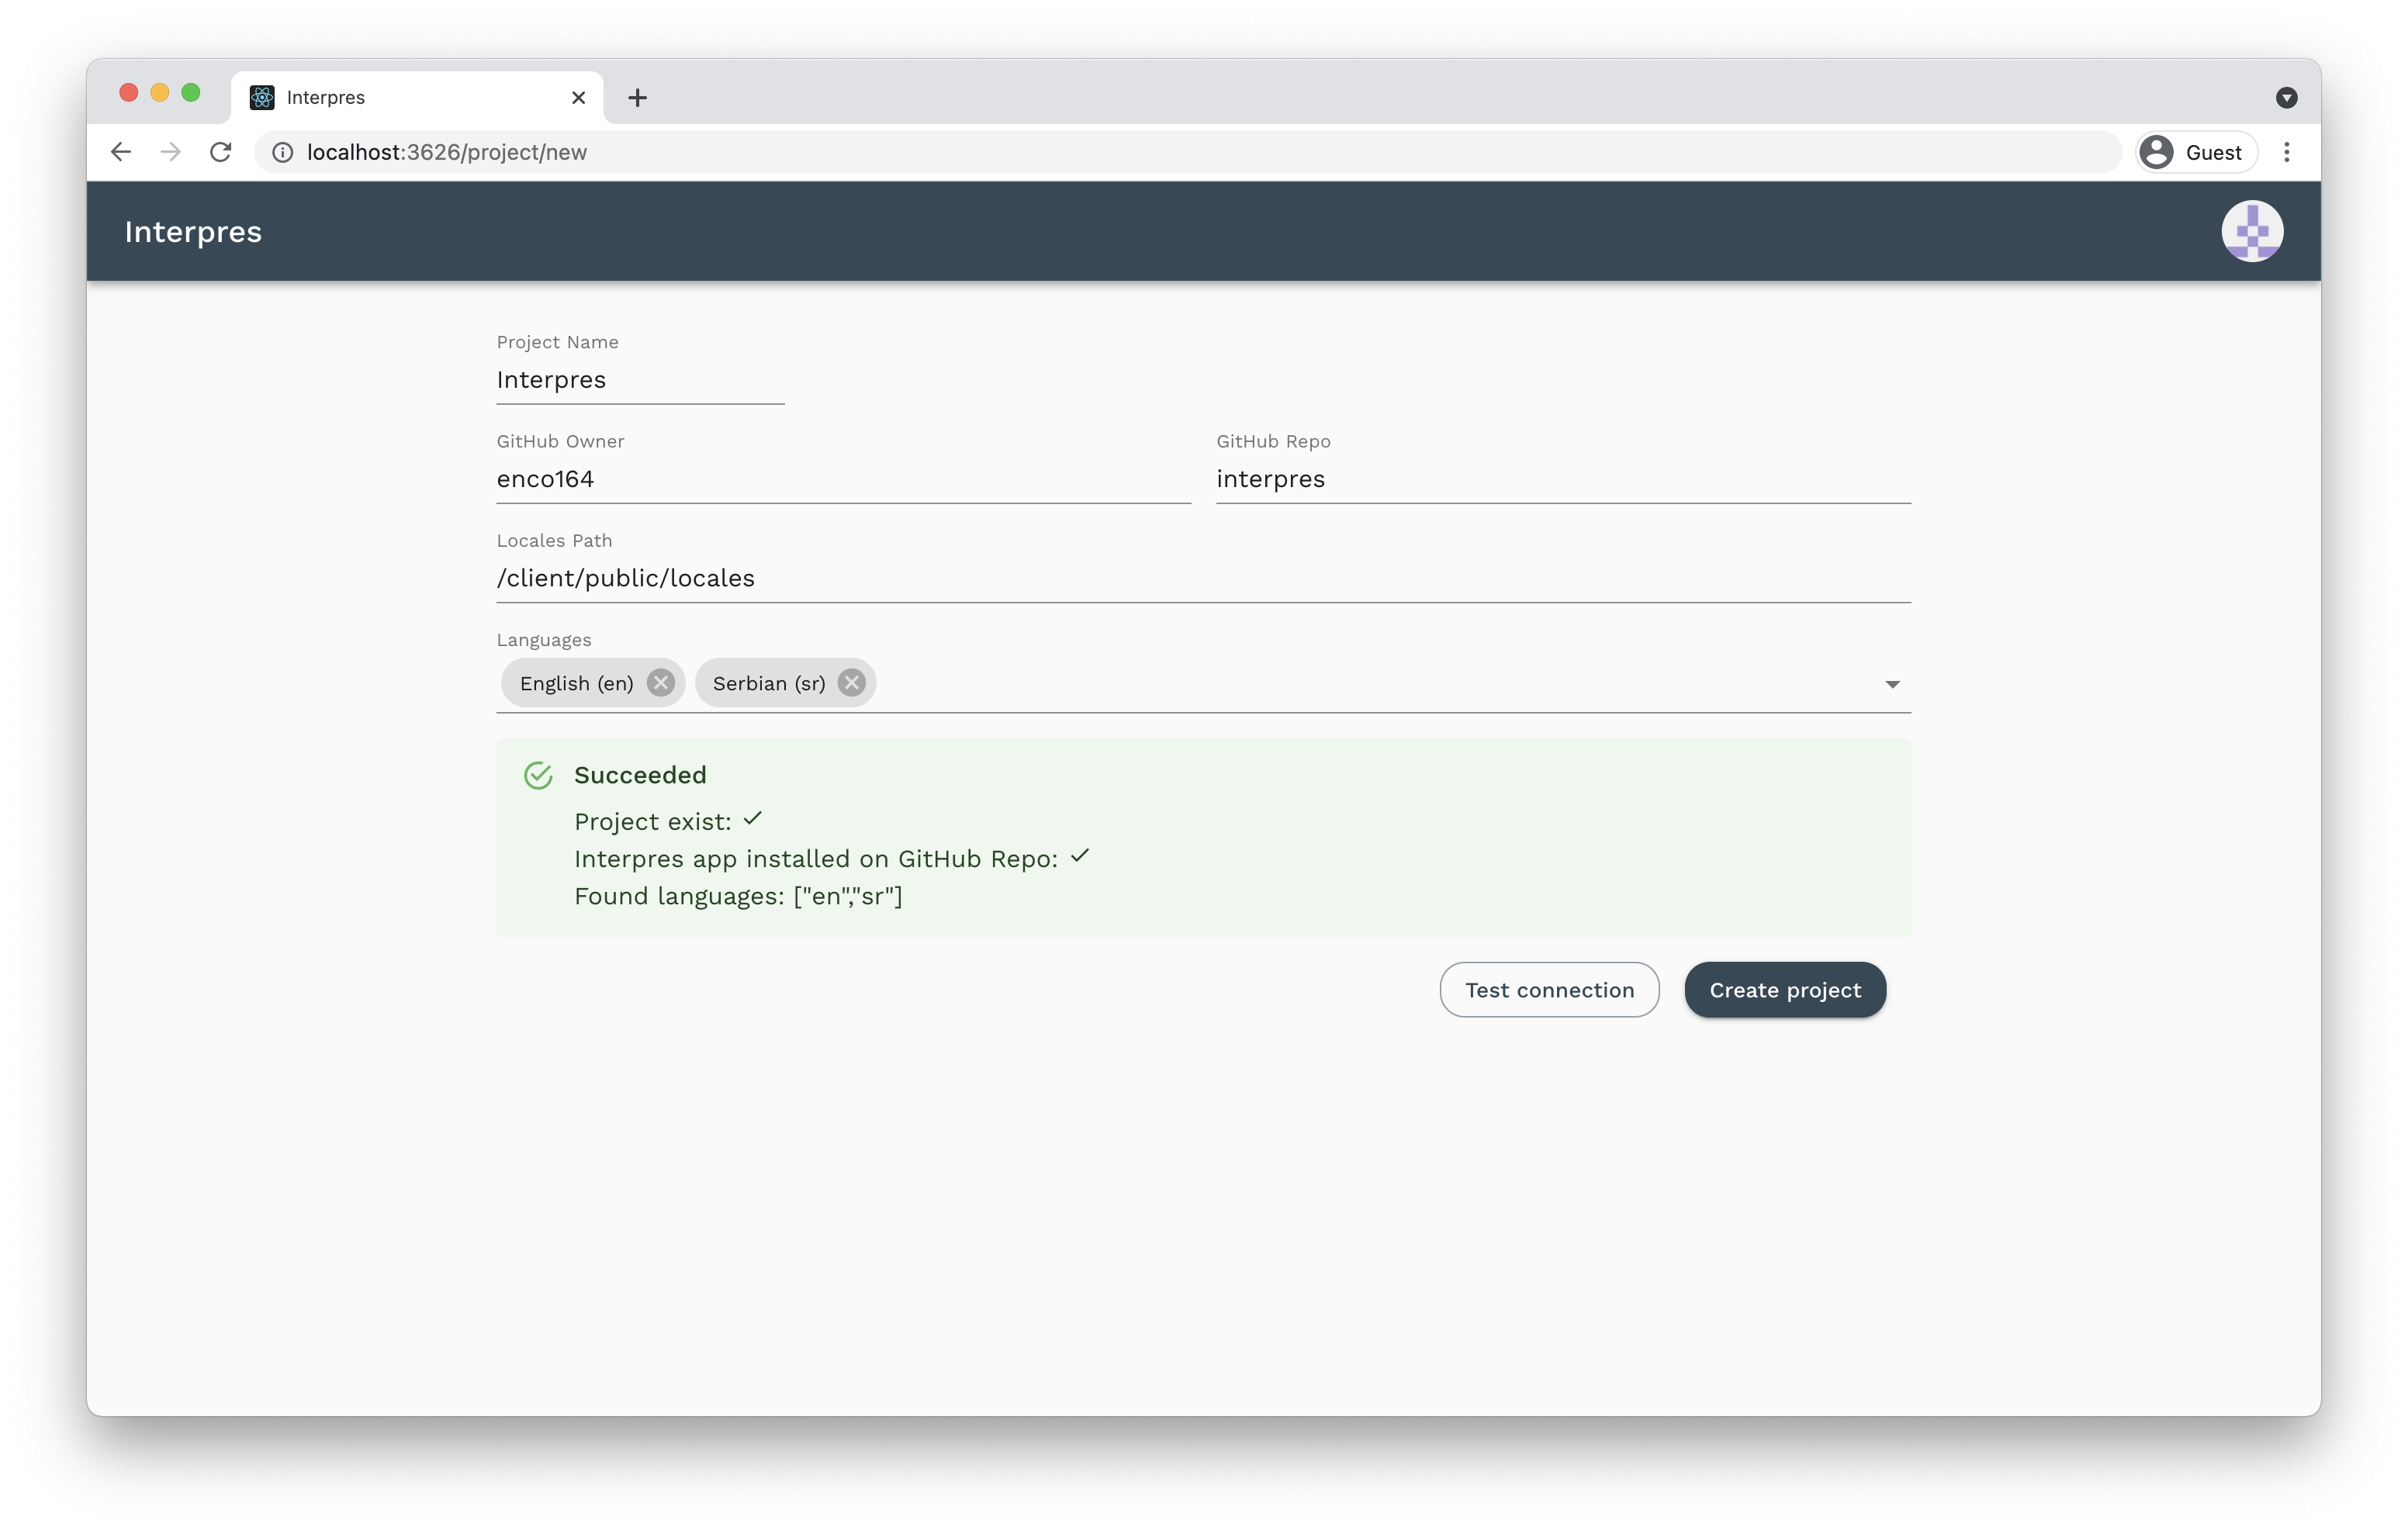
\includegraphics[width=1\textwidth]{create_project}
    \caption{Korisnički interfejs -- pravljenje projekta}
\end{figure}


%%%%%%%%%%%%%%%%%%%%%%
\section{Uvoz prevoda}

\textbf{Kratak opis}: Prevodilac želi da uveze prevode sa \textit{GitHub}-a

\textbf{Učesnici}: Prevodilac

\textbf{Postuslov}: Prevodilac se nalazi na projektu u koji želi da uveze prevode

\textbf{Glavni tok}:
\begin{enumerate}
    \item Sistem prikazuje opcije za uvoz i izvoz prevoda
    \item Prevodilac bira akciju za uvoz prevoda
    \item Sistem prikazuje modal sa porukom da će se uvozom prevoda sve 
    izmene koje nisu izvezene izgubiti
    \item Prevodilac klikne na dugme "\textit{OK}" ukoliko nema prevoda koji nisu sačuvani
    \item Sistem uvozi prevode
    \item Sistem zatvara modal
\end{enumerate}

\textbf{Alternativni tok}: Ukoliko prevodilac u koraku 5. klikne na dugme "\textit{Cancel}", 
sistem zatvara modal i prevodi neće biti uvezeni.


%%%%%%%%%%%%%%%%%%%%%%
\section{Izmena prevoda}

\textbf{Kratak opis}: Prevodilac vrši izmene kako bi dodao novi prevod ili izmenio postojeći

\textbf{Učesnici}: Prevodilac

\textbf{Postuslov}: Uspešno izvršena izmena prevoda

\textbf{Glavni tok}:
\begin{enumerate}
    \item Sistem prikazuje listu prevoda sa odgovarajućim ključevima
    \item Prevodilac klikne na željeni ključ za koji želi da unese ili izmeni prevod
    \item Sistem vraća tekstualna polja za unos za onoliko jezika koliko je u tom 
    trenutku dostupno za izabrani ključ
    \item Prevodilac unosi ili menja jedan ili više prevoda
    \item Prevod se automatski šalje na čuvanje u trenutku kada tekstualno polje izgubi fokus
    \item Sistem čuva izmenjeni prevod
\end{enumerate}

\begin{figure}[H]
    \centering
    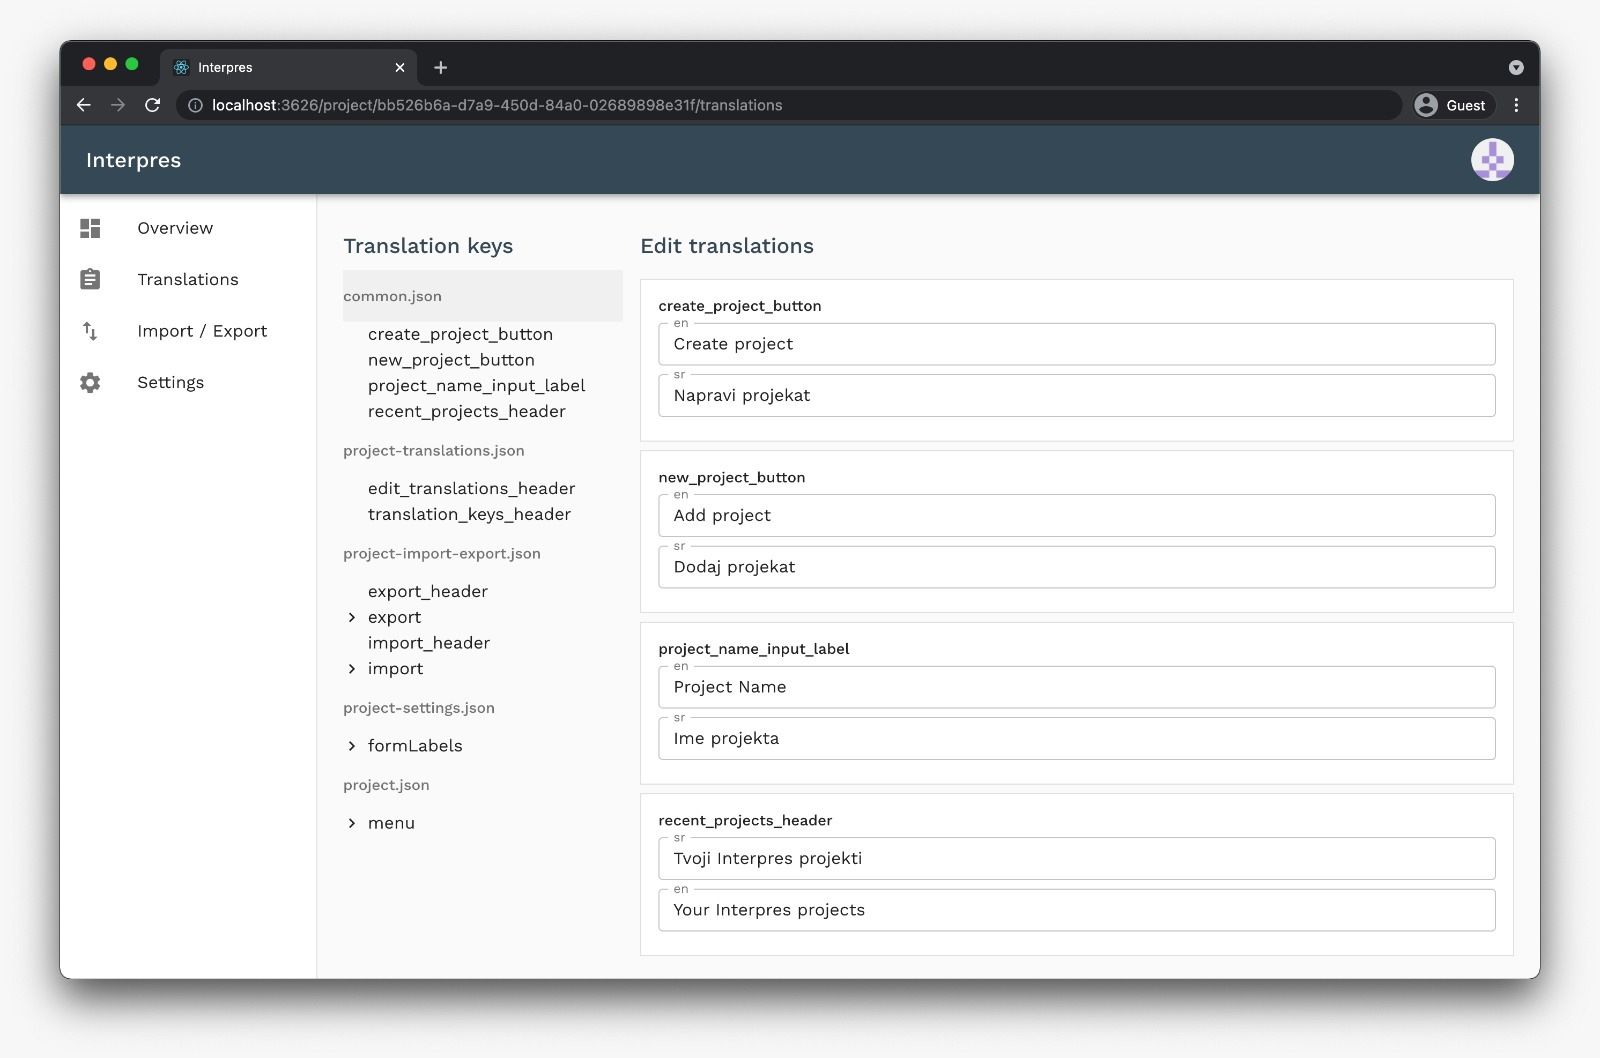
\includegraphics[width=1\textwidth]{translation_editor}
    \caption{Korisnički interfejs uređivača prevoda}
\end{figure}


%%%%%%%%%%%%%%%%%%%%%%
\section{Izvoz prevoda}

\textbf{Kratak opis}: Prevodilac želi da izveze prevode izabranog projekta i 
na taj način napravi zahtev za promenu na \textit{GitHub}-u

\textbf{Učesnici}: Prevodilac

\textbf{Preduslov}: Prevodilac se nalazi na projektu koji želi da izveze

\textbf{Postuslov}: Uspešno izvezen sadrđaj prevoda

\textbf{Glavni tok}:
\begin{enumerate}
    \item Sistem prikazuje opcije za uvoz i izvoz prevoda
    \item Prevodilac bira akciju za izvoz prevoda
    \item Sistem prikazuje modal sa formom za unos naslova i opisa 
    zahteva za promenu
    \item Prevodilac unosi naslov i opis u tekstualna polja
    \item Korisnik klikne na dugme \textit{OK}
    \item Sistem pokreće akciju izvoza prevoda
    \item Na \textit{GitHub}-u se pravi zahtev za promenu sa izmenjenim fajlovima za prevode
\end{enumerate}

\begin{figure}[H]
    \centering
    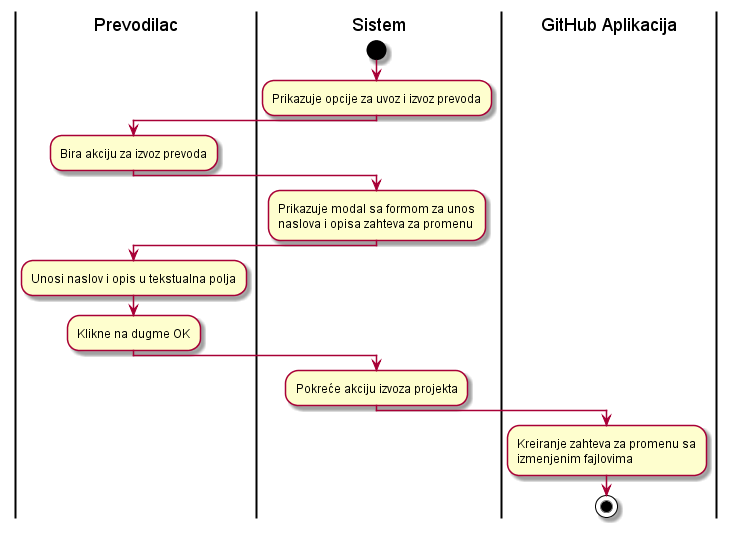
\includegraphics[width=0.7\textwidth]{izvoz_prevoda}
    \caption{Dijagram aktivnosti -- izvoz prevoda}
\end{figure}

\begin{figure}[H]
    \centering
    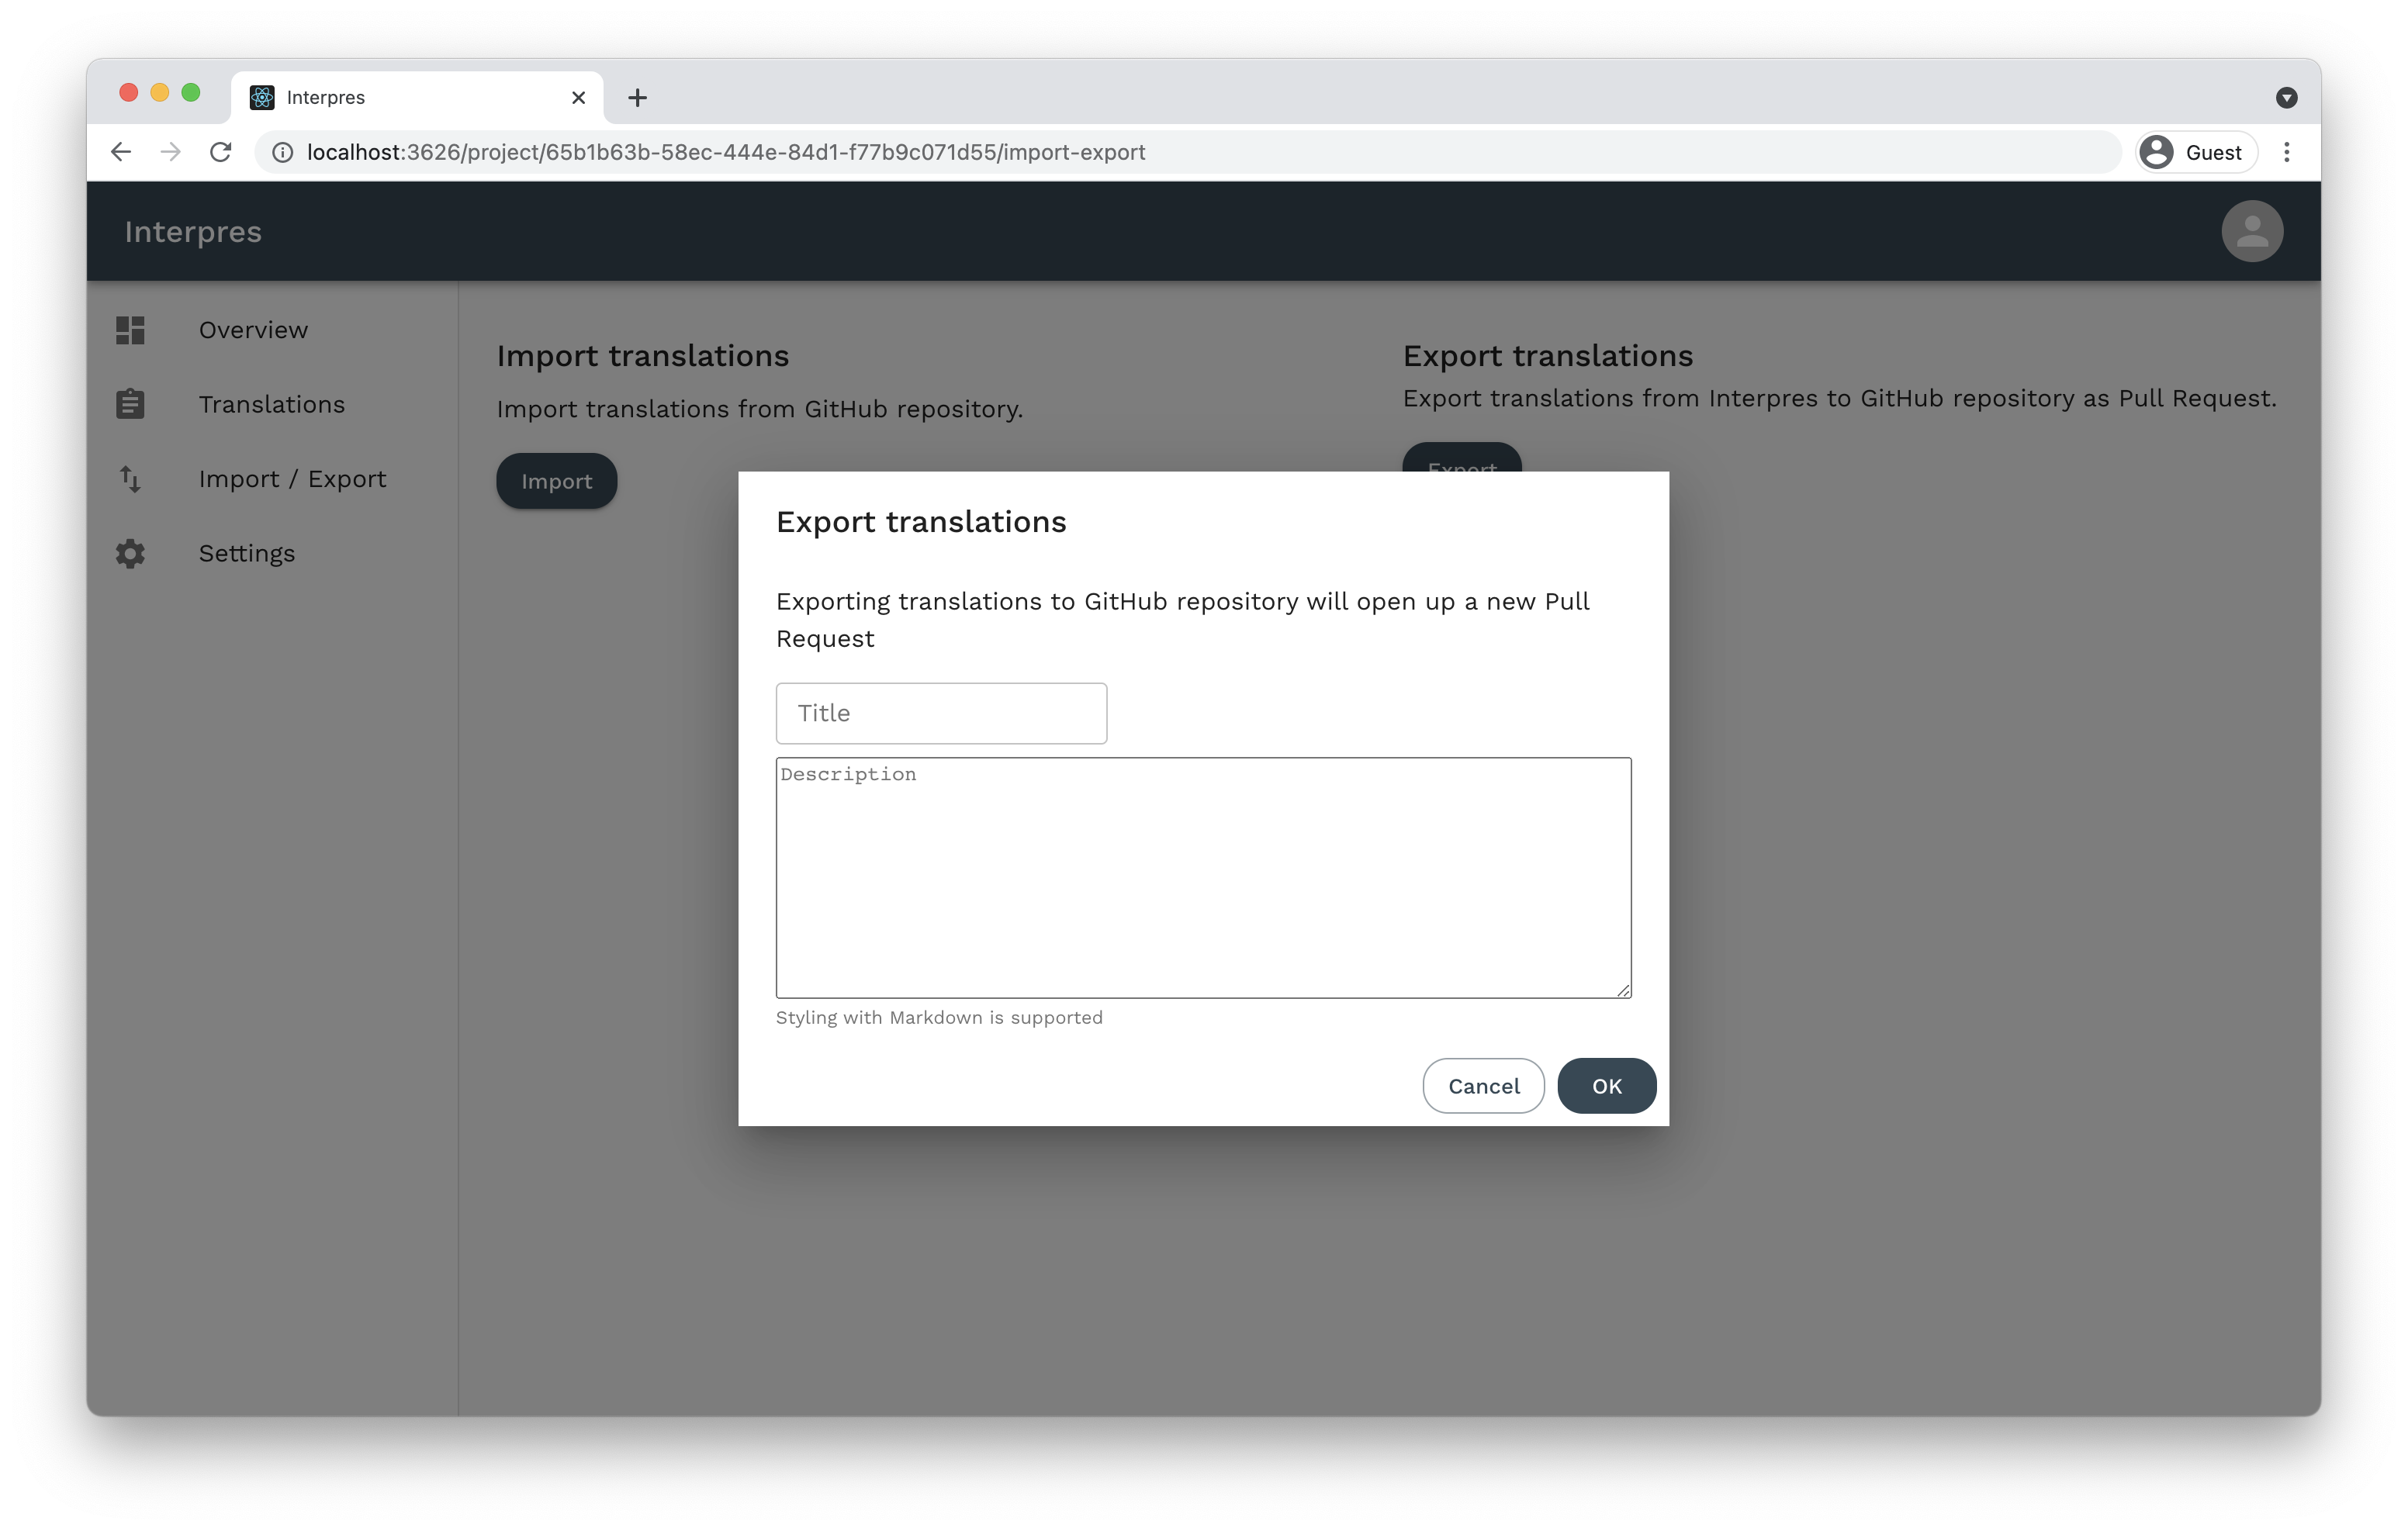
\includegraphics[width=1\textwidth]{export_translations}
    \caption{Korisnički interfejs za izvoz prevoda}
\end{figure}

